\chapter{Offline selection}
Decayed particles sometimes make fake trajectories and hits in the CDC and the CDH.
For expamle, neutral particles convert to charged particles at the solenoid magnets and these make hit in the CDH.
We select event by simple offline analysis to avoid these fake hits.

\section{$d(K^-, n \pi^+ \pi^-)$} \label{sec:software_select_kn}
Fig\ref{fig:CDH_time_dE} shows scatter plot of T0-CDH tof and energy deposit of the CDH by $\pi^+ \pi^-$ in $n_{forward}$ and $\pi^+ \pi^-$ detected events.
There are some events in slow region and low energy deposit region which will be fake events from low energy electron and decayed muon and so on.
We select time window of 1--15 [ns] to reject these fake hits.
Fig\ref{fig:CDH_dE} shows energy deposit of $\pi^+ \pi^-$ in smae events.
Red lines indicates energy deposit summed up clustering hits.
So, low energy deposit includes events that a pion pass through edge of the CDH.
We select two CDH clusters event accociating CDC tracks after hits filtered by time-window for $d(K^-, n \pi^+ \pi^-)$ events.
We also select energy deposit of the cluster more than 4.5 $[MeVee]$.

\begin{figure}[htbp]
  \centering
  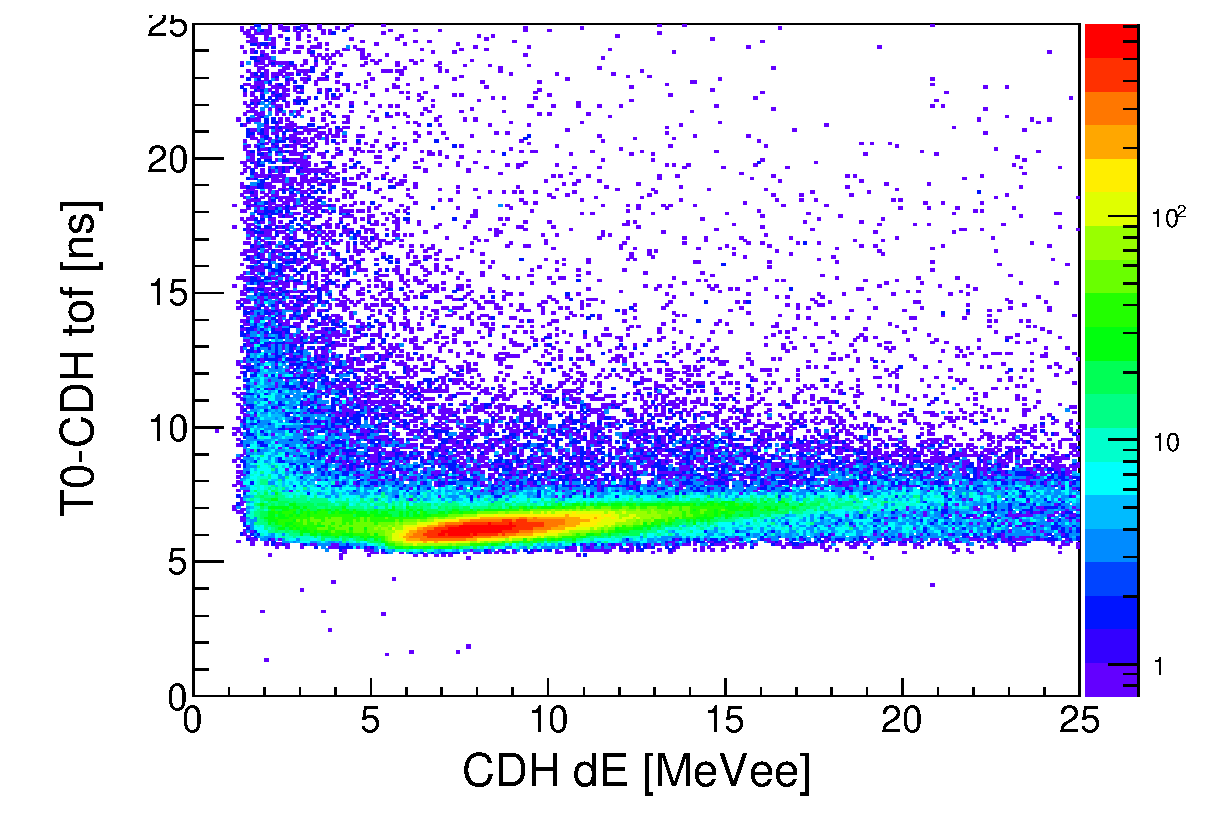
\includegraphics[width=6cm]{../pic/Dron/CDH_time_dE.eps}
  \caption{
   The figure indicates T0-CDH tof and energy deposit of the CDH of $\pi^+ \pi^-$ hits in $d(K^-, n \pi^+ \pi^-)$ events
  }
  \label{fig:CDH_time_dE}
\end{figure}

\begin{figure}[htbp]
  \centering
  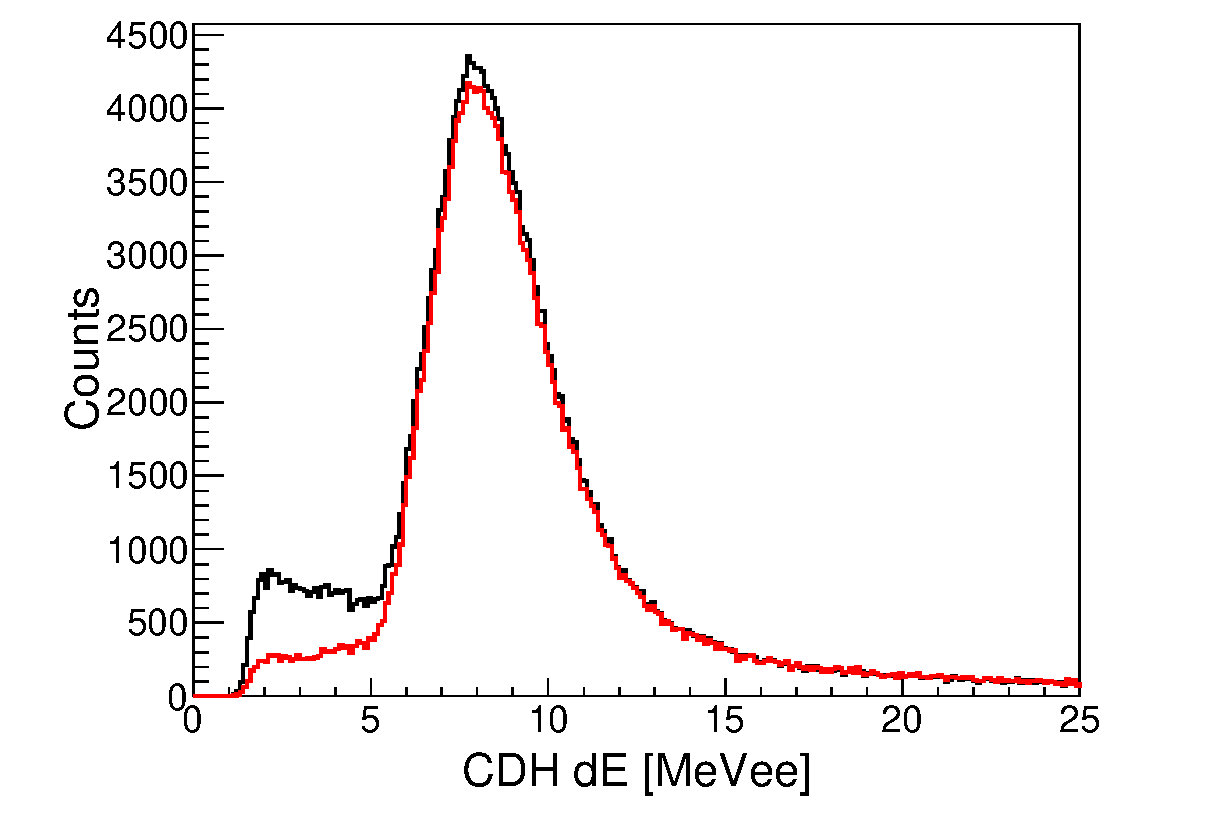
\includegraphics[width=6cm]{../pic/Run78/software/CDH_dE.eps}
  \caption{
    This figure shows $\pi^+ \pi^-$ energy deposit of the CDH in same condition of Fit\ref{fig:CDH_time_dE}.
    Black line indicate no selection and red line indicate clustering energy deposit.
  }
  \label{fig:CDH_dE}
\end{figure}

\section{$d(K^-, p \pi^- \pi^-)$} \label{sec:software_select_kp}
$d(K^-, p \pi^- \pi^-)$ event selection is same as $d(K^-, n \pi^+ \pi^-)$ event.
So, CDH hits were adopted timewindow and clustering as same as $d(K^-, n \pi^+ \pi^-)$ analysis which was shown in Fig\ref{fig:CDH_time_dE_kp}

\begin{figure}[htbp]
  \centering
  \begin{tabular}{cc}
    \begin{minipage}{0.5\hsize}
      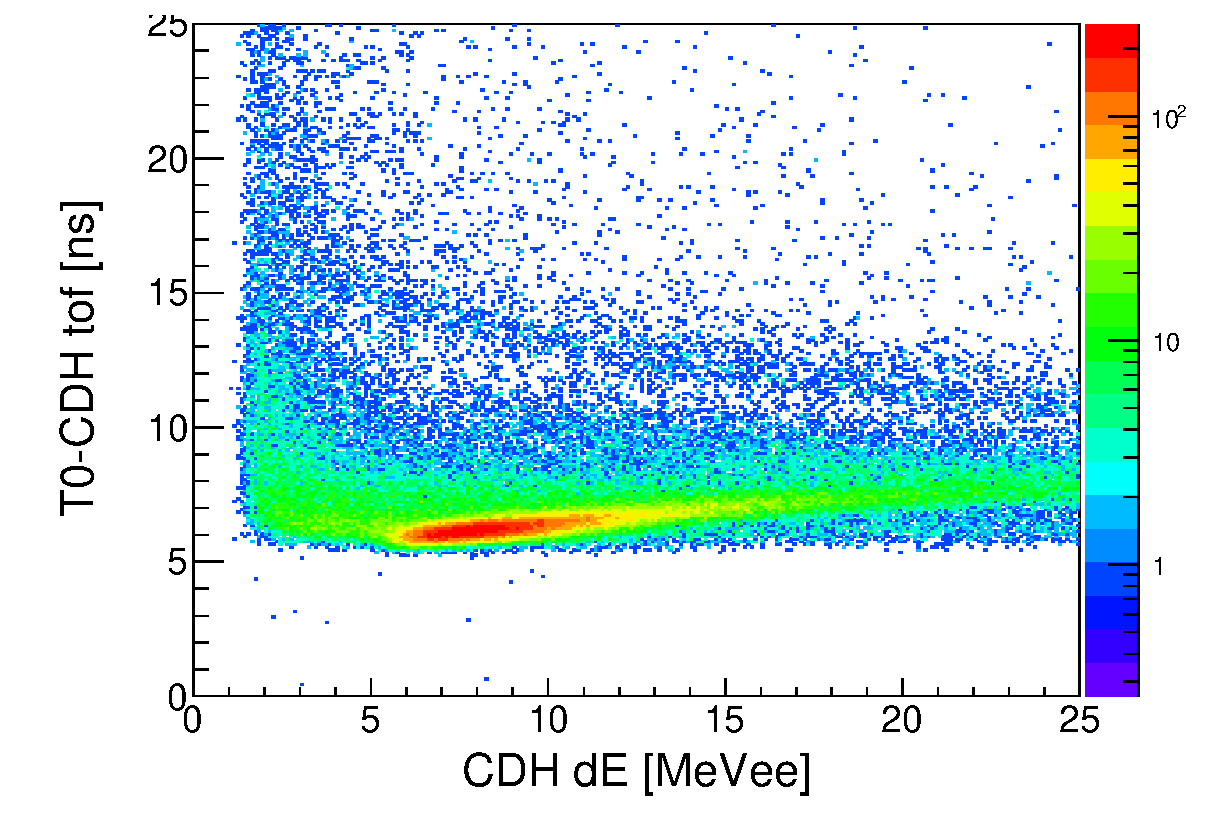
\includegraphics[width=6cm]{../pic/Dron/CDH_time_dE_kp.eps}
    \end{minipage}
    \begin{minipage}{0.5\hsize}
      \includegraphics[width=6cm]{../pic/Dron/CDH_dE_kp.eps}
    \end{minipage}
  \end{tabular}    
  \caption{
    These figures represent about offline selection for $d(K^-, p \pi^- \pi^-)$ events.
    Left figure shows scatter plot of T0-CDH tof and CDH dE in forward proton and 2 $\pi^-$ detected events.
    Right figure shows CDH dE in which black line indicates without clustering and red line indicates with clustering.
  }
  \label{fig:CDH_time_dE_kp}
\end{figure}
